
\chapter{Application of Graph Databases}

The workcell is considered a main building block of various industrial settings. Hence, it is examined as a primary testing environment for studying wireless communication techniques in factory automation processes. A new testbed was recently designed and developed to facilitate such studies in workcells by replicating various data flows in an emulated production environment. In this paper, an approach to storing and analyzing network performance data from a manufacturing factory workcell is introduced.  A robotic testbed was constructed using two collaborative grade robot arms, machine emulators, and wireless communication devices. A graph database approach was implemented to capture network and operational event data among the components within the testbed.  A schema is proposed, developed, and elaborated; a database is then populated with events from the testbed, and the resulting graph is presented. Query commands are then presented as a means to examine and analyze network performance and relationships within the components of the network.  Additionally, we demonstrate how to extract correlations between receive signal power and network delay within the testbed using the graph database query language.  Finally, using the inherently interconnected nature of the graph database, we discuss applying the graph database approach toward examining more complex relationships between the wireless communications network and the operational system.

\section{Introduction} \label{gdbappl:sec::intro}

% conceptual clarification
Wireless communication is a key enabling technology for the modernization of factory workcells. Modern factory workcells are highly-interconnected networked control systems in which various devices interact and collaborate to accomplish complex and adaptive production orders. The workcell often contains mobile robots that collaborate with other robots or human beings. Requirements of the workcell include the incorporation of mobile collaborative robotics with real-time coordination of motion and tool actuation.  As such, the communication of sensor and control information must be ultra-reliable and of low-latency to assure trustworthy operation~\cite{wirelessAutomation2017}. Due to an increased demand for ease of installation, reduced costs of deployment and maintenance, and flexibility, wired networks are being gradually replaced with wireless networks. This presents a real challenge for networks and control systems. Compared with wired connections, wireless links have their unique advantages in connecting field sensors and actuators with reduced cabling costs and natural support of mobility~\cite{ieMag2018}; however, most current communications systems lack the latency and reliability supports~\cite{etsi103588} mandated by factory owners~\cite{Industry40, SmartManuf}.  New wireless protocols are being designed to address reliability and latency concerns of real-time systems such as those in manufacturing automation.  These new protocols include advancements, such as the Institute of Electrical and Electronics Engineers (IEEE) 802.11ax standard and 5G cellular evolution as defined by the International Mobile Telecommunications-2020 (IMT-2020) Standard.  Both of these two standards employ improved diversity techniques for multiple access of devices as well as 1 ms latency and greatly improved reliability~\cite{80211ax}. 

Evaluation of such systems used in manufacturing environments requires not only rigorously analyzing  network performance, but also studying the impacts of networks on manufacturing systems. Additionally, industry lacks effective and easy-to-use strategies for test and evaluation of such systems in a way that correlates network performance with operational performance. Furthermore, since factory operators desire the ability to control operations within the workcell using wireless technology, we present a novel method to simultaneously capture network and operational event information using a graph database (GDB).  The use of a GDB allows for more intuitive inferences to be made through the stored relationships and graph theoretic models~\cite{Angles:2008:SGD:1322432.1322433}. In this paper, we present a GDB approach to the capture and analysis of factory workcell performance utilizing the Neo4j database platform. We present a proposed schema of the database, the process for capturing both network and operational events, and examples of querying the database for cyber-physical performance evaluation of the workcell for our collaborative two-robot machine-tending workcell\cite{Liu2019vancouver}.

\section{Graph Databases}
A GDB is the type of databases that uses nodes, edges, and properties to store and present data. A GDB is a part of a family of databases known as NoSQL databases that are used often to represent complex interrelated structures of data and their relationships.  This can be very difficult with traditional relational databases.  The GDB places a high priority on the relationships (edges) between units of information.  In addition, the GDB does not enforce any particular schema or structure, and, therefore, provides greater flexibility in storing and representing information in which the parts of information may vary among units. The relationships within a GDB are efficiently queried because they are persistently stored within the database.  In a GDB, queries can be made based on relationships. This, in particular, presents an advantage when storing information regarding systems with correlations that are apparent but difficult to visualize or quantify. The GDB approach was chosen for this specific purpose\textemdash{}to quantify and visualize relationships between non-ideal communications within a workcell and their impact on the physical system.

\section{Related Work}
Multiple surveys about GDBs have been presented to describe the associated models, tools, and their features in~\cite{Angles:2008:SGD:1322432.1322433,7148480,GDB_overview}. Also, examples of applications and implementations of GDBs are presented in~\cite{modern_models} to show their use on enterprise data, social networks, and determining security and access rights. It was found that GDBs provide the much needed structure for storing data and incorporating a dynamic schema. On the other hand, query languages are used to extract data including traversing the database, comparing nodes properties, and subgraph matching~\cite{Wood2012QueryLF}. The performance of different GDB tools and methodologies is analyzed and compared in~\cite{Jadhav2015ComparativeAO,Macko:2013:PIG:2485732.2485750}. Multiple comparisons in these articles have shown improved performance of Neo4j in the general features for data storing and querying, and data modeling features such as data structures, query languages and integrity constraints. 

Furthermore, industrial data analytics play an essential role in achieving the smart factory vision and improving decision-making in various industrial applications. Five main industrial data methodologies are studied including highly distributed data ingestion, data repository, large-scale data management, data analytics, and data governance~\cite{DBLP:journals/corr/abs-1807-01016}. Industrial data processing offers valuable information about various sections of industrial applications including inefficiencies in industrial processes, costly failures and down-times, and effective maintenance decisions~\cite{JLee}. In~\cite{4}, a platform for performing industrial big data analysis is presented where the performance requirements are introduced to achieve a cost-effective operation. Various other frameworks for industrial data analysis can be found in~\cite{5,6}, where the importance of using data analysis in decision making is emphasized.

Due to its advantages including scalability, efficiency, and flexibility, NoSQL databases are a popular alternative to relational databases in the case of large amounts of data in various applications~\cite{doi:10.1108/17440081311316398}. The GDB is a kind of NoSQL database approaches that additionally handles complex relationships~\cite{8123475}. GDBs are widely adopted in various industry-related applications and use cases such as network operations, fraud detection, and asset and data management~\cite{top5}. Relationships in social networks have been modeled using a GDB for structural information mining and marketing~\cite{Gomez-Rodriguez:2012:IND:2086737.2086741}. On the other hand, business solutions for scenarios with multiple large data sources require distributed processing in decision making for various problems such as fraud detection, trend prediction, and product recommendation~\cite{Skhiri2013}.

\section{Case Study: Robotic Machine-tending}
In this section, we present a two-robot machine tending workcell case study.  We first present the design of the workcell followed by an elaboration of the database design called a schema.  The information work-flow, i.e., the process for collecting, processing, and analyzing the network event data is presented.  We then provide examples of the resulting graph and results of targeted queries that demonstrate the purpose of the database. 
\subsection{Workcell Design}

\begin{figure}[!ht]
	\centering
	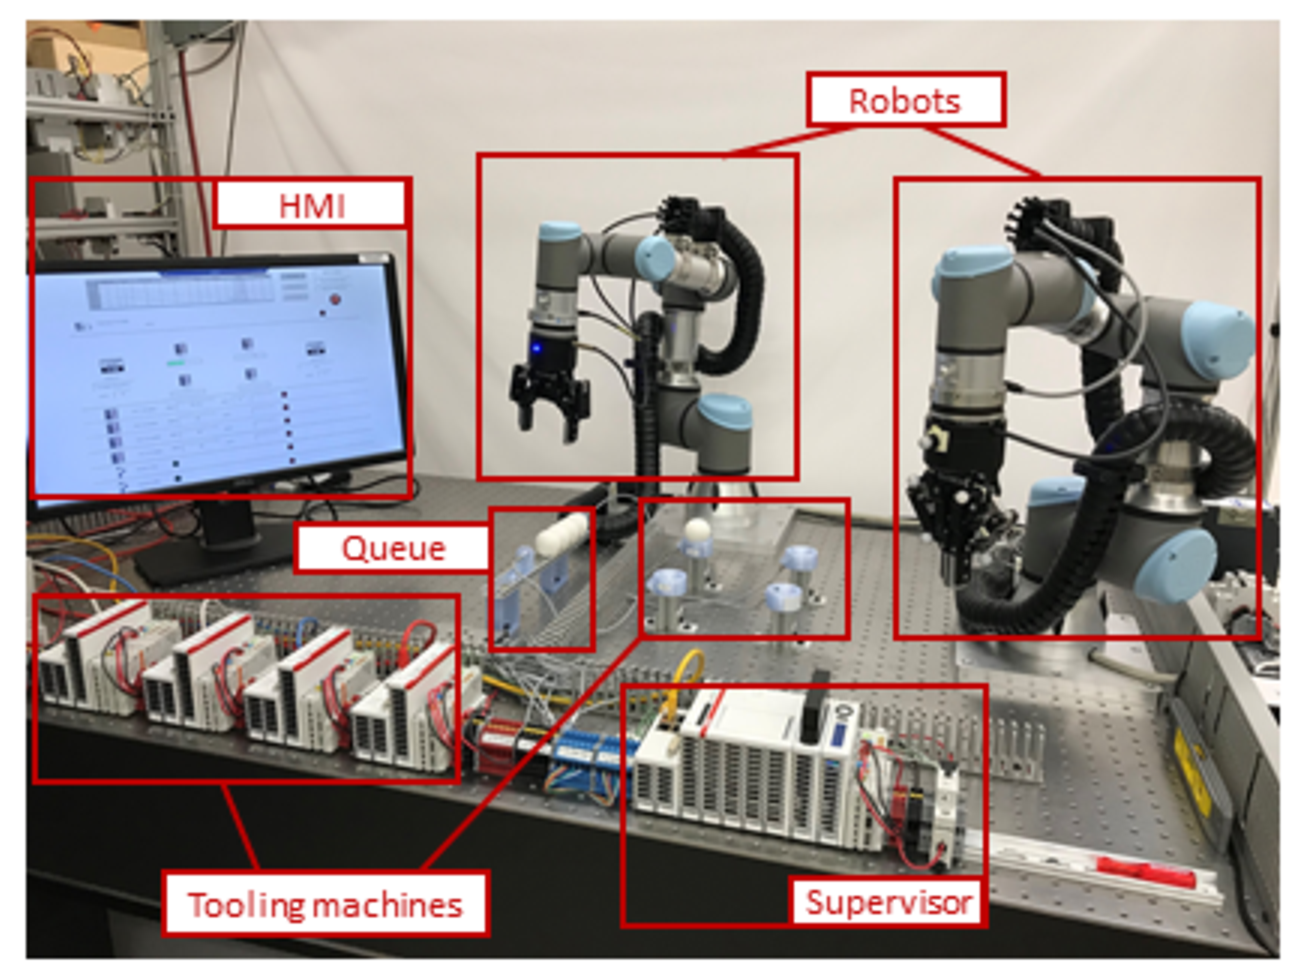
\includegraphics[width=\textwidth]{./chapter-gdb-appl/figures/cellShot}
	\caption{Collaborative work cell testbed}
	\label{gdbappl:fig::workcell}
\end{figure}

To facilitate wireless network research and showcase the power of wireless technologies in industrial practices, a testbed shown in Fig.~\ref{gdbappl:fig::workcell} has been developed at the National Institute of Standards and Technology (NIST) as described in~\cite{Liu2019vancouver}. The testbed is composed of two collaboration-grade robots, a supervisory programmable logic controller (PLC) used for the control of the workcell, four smaller PLCs serving as computer numerical control (CNC) machine emulators, and a human-machine interface (HMI).  Each robot is equipped with a six-degrees-of-freedom (DOF) force-torque (FT) sensor and a two-finger gripper. A Modbus/TCP server is included within the supervisor PLC and is used for communication between the supervisor and the robots.  The PLCs themselves communicate to each other using the Beckhoff Automation Device Specification (ADS) protocol. All elements within the workcell are synchronized to a stable and accurate grand-master clock. Therefore, as described in~\cite{Liu2019vancouver}, the operational, network, and measurement elements are all synchronized to the grand-master clock through a precision time protocol (PTP)-capable switch. 

Work-orders for the workcell are submitted through the supervisor. Each work-order consists of a work-plan for a part, and the work-plan determines how each part moves through the workcell until it is completed. The inspection of each part is conducted at each machining station, and after the final inspection, the part is placed back into the input queue.  Under normal operating conditions, the work continues until all work-orders have been processed.  This continuous form of operation provides ample opportunity to collect statistically significant metrics of both the network and the operation of the workcell.

\subsection{Database Schema}\label{gdbappl:sec::dbschema}

\begin{figure}[!ht]
	\centering
%	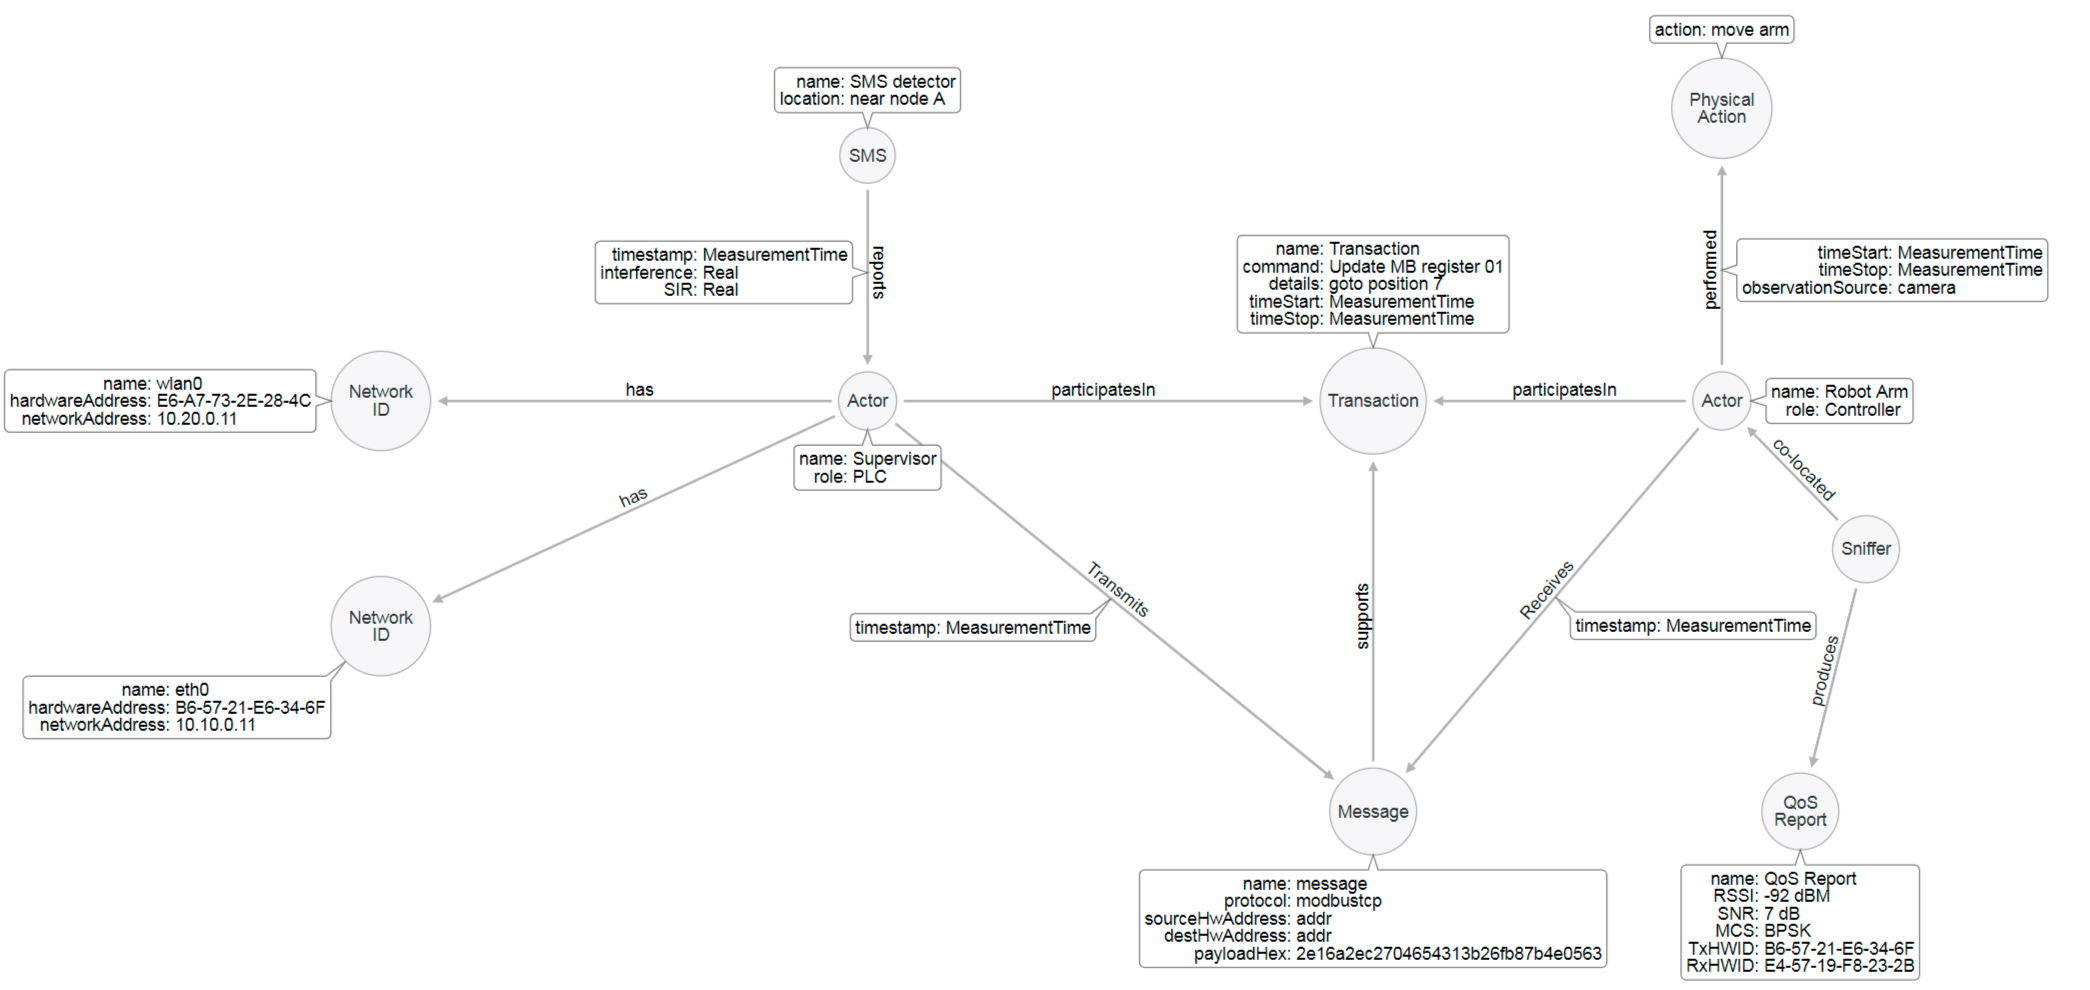
\includegraphics[width=\textwidth,trim=50 50 50 50, clip]{figures/database/arrows-schema.PNG}
	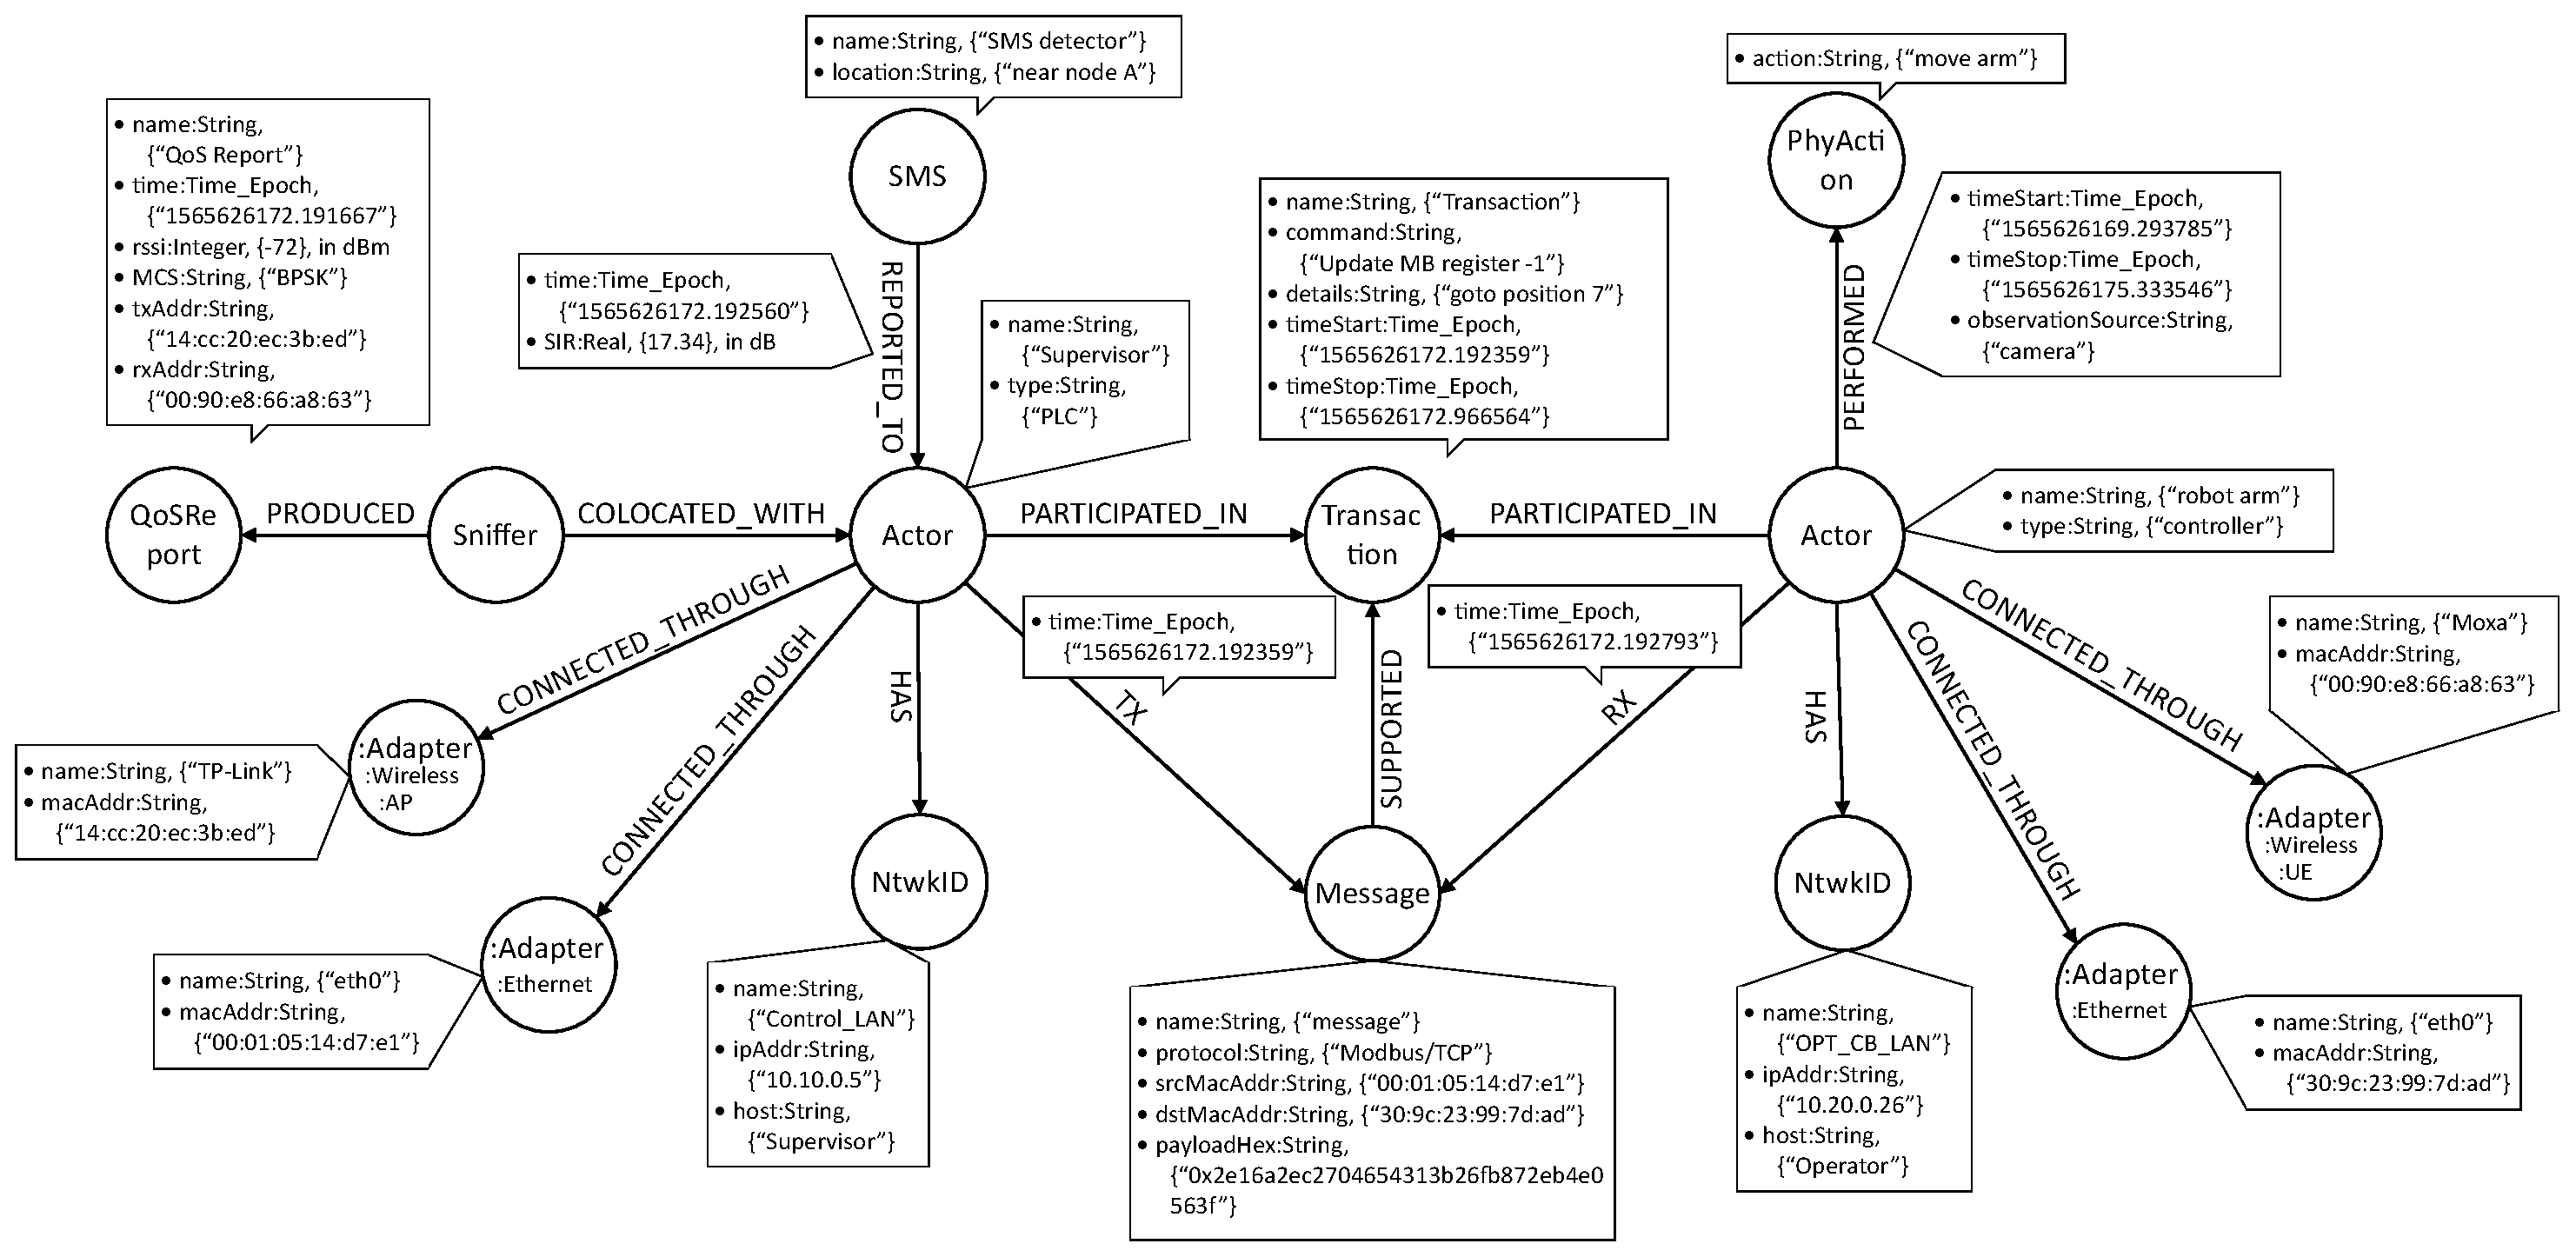
\includegraphics[width=\textwidth]{./chapter-gdb-appl/figures/database/graph_schema_0816.eps}
	\caption{The intended schema (i.e., pseudo-schema) of the graph database used for each operational run of the NIST wireless factory testbed.  The graph is organized into nodes and edges, where the edges signify relationships among network elements and physical operational elements.}
	\label{gdbappl:fig::database:schema}
\end{figure}

GDBs are NoSQL databases such that the database does not contain any predefined structure or rules to enforce such structure.  This is a major difference between relational databases and GDBs.  Nevertheless, it was necessary to sketch a pseudo-schema to capture the intended nodes and relationships that would be stored within the database (the terms pseudo-schema and schema will be used interchangeably). Before describing the schema itself, it is necessary to first explain the requirements of the schema.  Therefore, the requirements for our schema are as follows:

\begin{description}[style=sameline]
% [Time] 
\item[Time] Any manufacturing automation system is indeed a time-varying control system with network and operational events.  The database schema must necessarily support time-based queries and, specifically, time-windowed 
queries.
% [Operational Events]
\item[Operational Events] The schema must represent operational events such as the movement of a robot arm or the movement of a part.
% [Network Events]
\item[Network Events] The schema must represent network events such as the transmission of packets.
% [Transactions/Grouping]
\item[Message Grouping]  The schema must support grouping of logically related events such that those events can be correlated to a specific occurrence within the testbed.
% [Wired/Wireless Support]
\item[Wireless Support] The schema must support the capture of both wired and wireless network traffic without special provisions within queries for either.
% [QoS]
\item[QoS Support] The schema must allow for the capture of quality of service (QoS) data when available.
% [Spectrum Monitoring]
\item[Spectrum Monitoring] The schema must support the capture and association of network events with observations from a spectrum monitoring system (SMS) if that information is available.
\end{description}

\subsubsection{Node Design}

Given the fore-mentioned requirements, a sample pseudo-schema is shown in Fig.~\ref{gdbappl:fig::database:schema}, which represents the intended structure of the information within the GDB. It is important to remember that since GDB schemas are not really schemas, such as those found in relational databases, but representations of intent, the schema represented here should be considered a notional example of the final product.  Within the graphs, nodes represent logical elements, and edges represent the relationships between those elements.  Both nodes and edges may contain properties providing more description and labels that define categories or classes of the said nodes or edges.  Our schema is designed such that the data within the graph is intuitive to understand and allows for time-based queries to occur.  The facilitation of time-based queries was an essential requirement of our database design.  Our schema is represented using the following node labels:

\begin{description}[style=sameline]
    \item[Actor]  A physical component within the factory workcell such as a robot, PLC, or other networked item.
    \item[NtwkID] A network address item for an actor such as an Internet Protocol (IP) address.
    \item[Transaction] A complete information exchange between two or more actors (multiple actors may participate in a transaction).
    \item[Message] A network transmission event that occurs between two actors (messages are essentially packet transmissions captured at the transport layer; multiple messages support a transaction).
    \item[Physical Action]  A physical occurrence within a factory workcell associated with actors through multiple time based relationships.
    \item[SMS] An SMS observes and records significant spectral events within the workcell and may report those events to actors within the workcell.  
    \item[Sniffer] A measurement device that records all transmissions conducted over the wireless medium and includes wireless header information for each wireless transmission detected.
    \item[Adapter] A device that serves to connect an actor to a network (adapters are divided into sub-categories depending on the type of interface to a network).
    \item[Adapter:Ethernet] A subcategory of adapter representing an Ethernet interface. 
    \item[Adapter:Wireless] A subcategory of adapter representing a wireless interface. 
    \item[Adapter:Wireless:AP]  A subcategory of adapter representing a wireless access point interface.
    \item[Adapter:Wireless:UE] A subcategory of adapter representing a wireless user equipment interface.
    \item[QoS Report] A quality of service report of a message (not all messages will have a QoS report).
\end{description}

It is important to note that most network infrastructure components are not captured within the graph, but, instead, only basic interfaces between actors and the network are captured.  Our intent when designing the graph was to make the graph network and protocol agnostic, such that the network is viewed as a black-box. Accordingly, the captured events of the physical system and the network are considered useful for the analysis of performance. 

\subsubsection{Relationships (Graph Edges)}
Relationships are edges within the graph that capture the informational interactions between nodes.  Relationships, like nodes, can contain labels and properties.  As shown in Fig.~\ref{gdbappl:fig::database:schema}, nodes are connected through defined relationships.  A subset of the relationships are defined as follows:
\begin{description}
    \item[PARTICIPATED\_IN] Actors will participate in transactions.  A transaction exists for each logical set of messages between actors such as the setting of a Modbus register or the sending of a command to a robot.  Therefore, actors will participate in many transactions, and multiple actors may participate in a single transaction.
    \item[SUPPORTED] Messages (i.e., packets between actors) are associated with transactions through the SUPPORTED relationship. Depending on the protocol and the quality of the channel, a single transaction could have one or many messages connected through this relationship.
    \item[TX/RX] An actor may either transmit (TX) or receive (RX) a message. Both the TX and RX relationships contain a timestamp in the format of an epoch time which is a floating point number in seconds since January 1, 1970, with a resolution of microseconds.
    \item[PERFORMED] When an actor performs a physical action, a relationship is created between the actor and the physical action node. This relationship contains start and stop time properties as well as the source of the observation such as a networked camera.
    \item[REPORTED\_TO] An SMS may be a passive or active listener within a workcell.  When an SMS operates as an active listener, spectral reports from the SMS may be sent to an actor such that the actor can respond intelligently to the spectral event.  Reports from an SMS to an actor are captured within this relationship.
\end{description}
Other relationships shown in the schema of Fig.~\ref{gdbappl:fig::database:schema} but not explained above are considered self-explanatory.

\subsubsection{Closer Examination}
Examining the sample schema more closely, two actor nodes are represented.  In this case, Actor A is the supervisory controller, and Actor B is a robot arm.  Both nodes participate in a transaction, which, in this example, is a Modbus/TCP exchange. The transaction itself is associated with one or more messages (i.e., packets). Each message associated with a transaction manifests itself as a node in the graph. Multiple message nodes will exist for each transaction. 
%It is important to note that a timestamp is not recorded for each message.  The reason is that the timestamp for a message is captured in the edge relationships between the sender and the message and the receiver and the message.  Thus, a timestamp for transmission and reception are recorded within the graph through the TX/RX relationships.  
Additionally, QoS reports may be associated with each actor node through a collocated sniffer node.  By keeping QoS reports separate, we have the flexibility of supporting different wired and wireless protocols within the same graph. Recall, that a graph database has no enforceable structure and thus affords this type of flexibility. Each actor node may have network identities associated with it through the use of network identifier nodes.  Each network identifier node may contain address information such as a hardware address or a network address; however, this is dependent on the protocols and addressing schemes being used, and a node could have many different identification nodes. 
\subsubsection{Physical Actions}
Finally, each actor in the graph may associate with physical actions.  These actions exist in the database as automatons such that every time a new action occurs, a new edge would be added between the actor and the physical action.  Timestamps within the graph represent ``measurement time'' denoting that all  timestamps are accurately synchronized to the grand-master clock.  The method of synchronization is outside the scope of this paper and is explained fully in~\cite{Liu2019vancouver}.  This paper describes the database structure and the process for preparing and inserting the data into the database, which is described in the following subsection.

\subsection{Information Workflow}

\begin{figure*}[!ht]
    \centering
    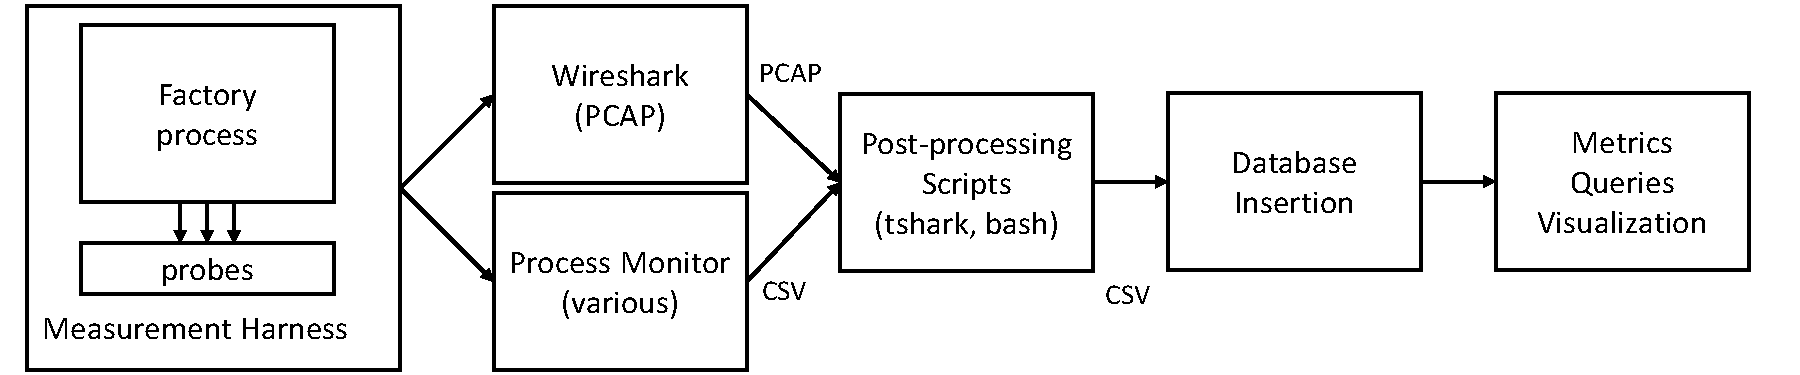
\includegraphics[width=0.95\textwidth]{./chapter-gdb-appl/figures/database/work-flow.pdf}
    \caption{Data processing flow from factory workcell to database}
    \label{gdbappl:fig::work-flow}
\end{figure*}

The workflow for collecting, processing, and inserting measurement data into the graph database is multi-pronged, as shown in Fig.~\ref{gdbappl:fig::work-flow}.  The workcell, which in our case study is a two-robot workcell with four CNC machines, is instrumented with network probes that capture transmitted and received packets as well as probes to capture operational movements such as arm robot position and the state of the supervisor PLC.  Network data is stored in packet capture (PCAP) files, while operational data is stored in comma separated value (CSV) files. We developed bash scripts to extract relevant information and prepare the data for insertion into the database. The scripts also contain rules for grouping packets together as transactions based on the application protocol and time. The scripts produce CSV files that are ready for insertion into the Neo4j database.  Once the data resides within the database, we apply queries to extract information for the evaluation of workcell performance and visualization of network and operational events within the workcell. By tracking paths through the relationships within the graph, discerning how a network event such as interference is related to physical events such as position uncertainty or part throughput is possible. Various impairments may be introduced as a part of workcell operation.  Examples of such impairments include competing wireless traffic, radio interference, and reflections and diffraction due to the multi-path environment~\cite{Candell2017.NIST1951}. We have shown that it is feasible to implement such impairments and measure the resulting physical performance manifestation~\cite{Liu2019vancouver}. This is accomplished through the use of a radio channel emulator as demonstrated in~\cite{Candell2019vancouver}.

\subsection{Sample of a Resulting Graph}
In the following, we show results from a trial run of the NIST industrial wireless testbed. In this trial run, a single physical wireless link is used between a wireless adapter connected directly to the supervisor and a wireless access point connected to all the other actors in the testbed. The wireless nodes represent IEEE 802.11b/g/n devices and are connected through a variable radio frequency (RF) attenuator that allows us to vary the channel quality. During the trial run, the production of 10 parts was emulated, which resulted in 10 minutes of network activity.       

After populating the database with data captured from the trial run, the resulting realized schema is shown in Fig.~\ref{gdbappl:fig::real-schema}. The schema visualization is produced by invoking the command

\begin{lstlisting}
call db.schema.visualization()
\end{lstlisting} 
in Neo4j. It is important to note that a realized schema shows only one representation of each node and relationship whereas the intended pseudo-schema shown in Fig.~\ref{gdbappl:fig::database:schema} was developed to exemplify the relationships between types of nodes, labels, and relationships. Where label inheritance is employed, such as the case for different adapter types, relationships are reproduced; however, this is a result of the visualization tool rather than the schema itself.  Fig.~\ref{gdbappl:fig::real-schema} serves, therefore, to validate that the intended schema was indeed realized by the insertion of event data from the testbed. In the realized schema, inherited labels are shown as separate nodes.

\begin{figure}[!ht]
    \centering
    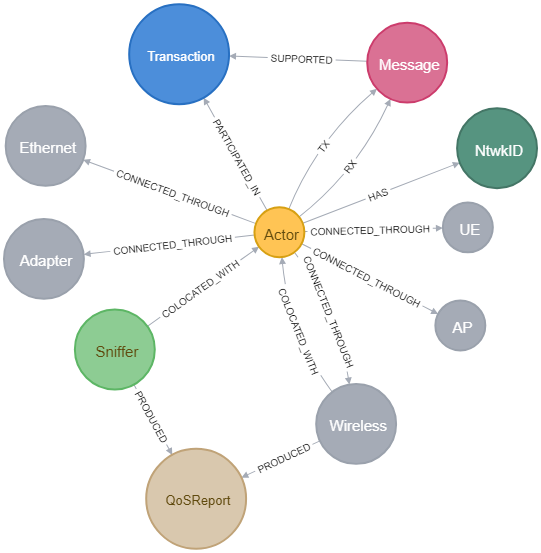
\includegraphics[width=0.99\columnwidth]{./chapter-gdb-appl/figures/database/graph_schema.png}
    \caption{Realized schema of the graph database fully populated after capturing network and operational data from the NIST industrial wireless testbed. }
    \label{gdbappl:fig::real-schema}
\end{figure}

As described in Section~\ref{gdbappl:sec::dbschema}, the database includes every network transaction that occurs during the operation of the testbed.  This includes any logical transaction nodes inserted into the database and any associated packets that happened to traverse the network.  Therefore, for a short duration of time depending on packet transmission rates, the amount of data stored in the database can grow quickly. This presents a visualization challenge that graphs are designed to handle. A sample graph is shown in Fig.~\ref{gdbappl:fig::Sample-graph_1}, which represents only 1 second of wired and wireless network data captured from the NIST two-robot pick-and-place wireless testbed described in~\cite{Liu2019vancouver}. 

\begin{figure}[!ht]
    \centering
   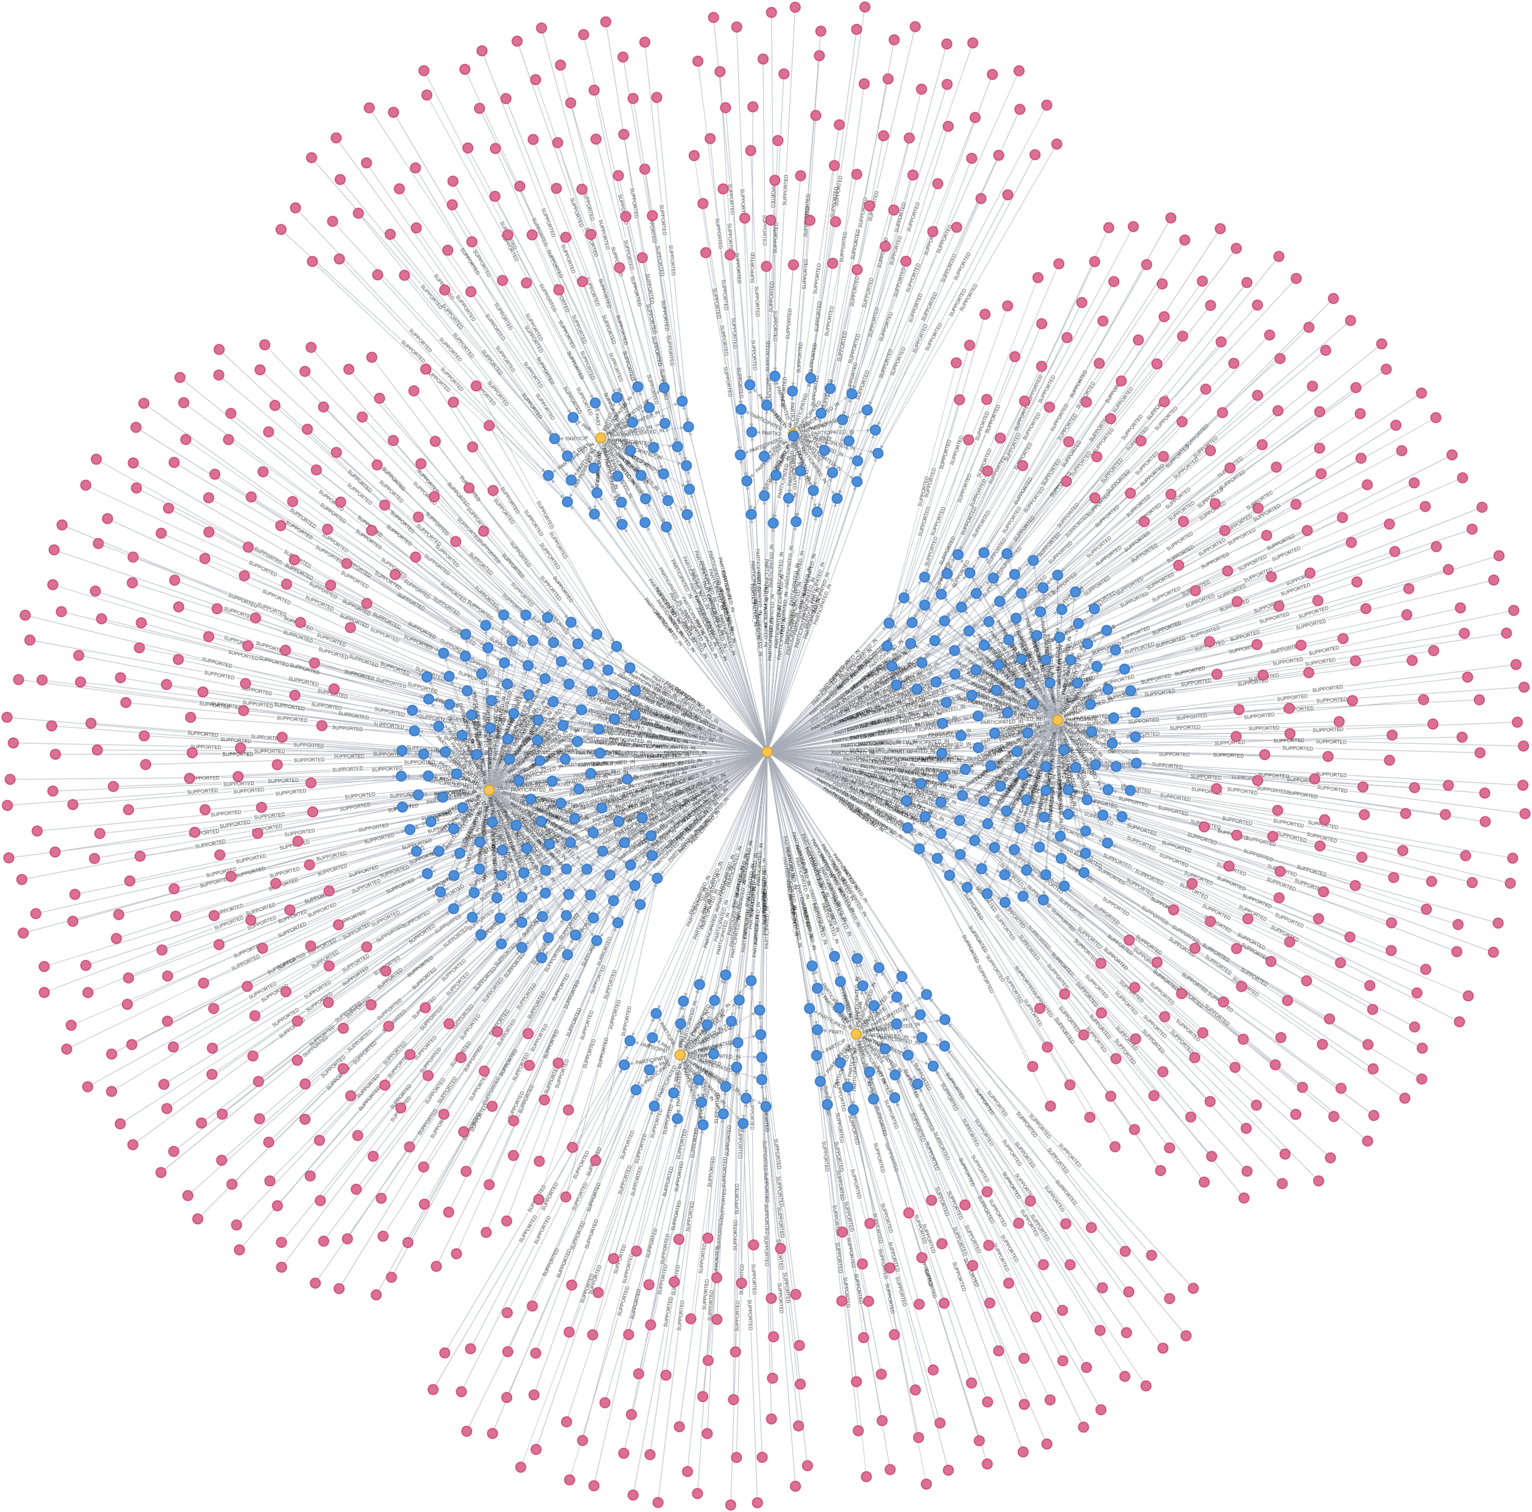
\includegraphics[width=0.95\textwidth]{./chapter-gdb-appl/figures/database/graph_M_T_2.png}
   \vspace{0.1in}
    \caption{ Visualization of a node graph resulting from a testbed experiment. }
    \label{gdbappl:fig::Sample-graph_1}
    \vspace{0.1in}
\end{figure}

This visualization is produced by calling the following query in the Neo4j. 
\begin{lstlisting}
MATCH p=(a:Actor {name:'Supervisor'})--(t:Transaction)--(b:Actor) ,p2=(m:Message)-->(t) WHERE t.timeStart>T AND t.timeStop<T+1
RETURN p,p2
\end{lstlisting}

The colors of the resulting nodes follow the realized schema in Fig.~\ref{gdbappl:fig::real-schema} while only the actors, transactions, and messages are visualized in Fig.~\ref{gdbappl:fig::Sample-graph_1}. The relationships between the messages and transactions are shown where a single transaction is connected to at least two messages to represent the communications between any two actors. The variable T in the query represents an arbitrary time variable in seconds within the trial run to capture the data within 1 second only.

We then show a more detailed visualization for all the nodes and relationships corresponding to a single transaction. This visualization is produced by calling the following query where Ts is an arbitrary time variable to specify the timeStart value for the single transaction. 

\begin{lstlisting}
MATCH p=(a:Actor {name:'Supervisor'})-->(t:Transaction {timeStart:Ts})<--(b:Actor {name:"CNC-1"})
WITH p, a, b, t
MATCH p1=(a)-->(m:Message)<--(b), p2=(m)-->(t), p3=(a)-[:HAS]-(),p4=(a)<-[:COLOCATED_WITH]-()-[:PRODUCED]->(q:QoSReport), p5=(a)-[:CONNECTED_THROUGH]-(),p6=(b)-[:HAS]-(), p7=(b)-[:CONNECTED_THROUGH]-()
WHERE q.time>t.timeStart AND q.time<t.timeStop
RETURN p,p1,p2,p3,p4,p5,p6,p7
\end{lstlisting}

In Fig.~\ref{gdbappl:fig::Sample-graph_2}, the actor nodes are labeled by their names \textit{CNC-1} and \textit{Supervisor}, the transaction is labeled by its type \textit{ADS}, the messages are labeled by their transmission role \textit{Request} and \textit{Response}, the NtwkIDs are labeled by their IP addresses, the Ethernet adapters are labeled by their names \textit{eth0}, the wireless adapters are labeled by their names \textit{Moxa} and \textit{TP-Link}, the sniffer is labeled by its name \textit{WLS1}, and the QoS reports are labeled by the received signal strength indicator (RSSI) value in dBm. This visualization includes only the QoS reports generated within the duration of the corresponding transaction.   

\begin{figure}[!ht]
    \centering
    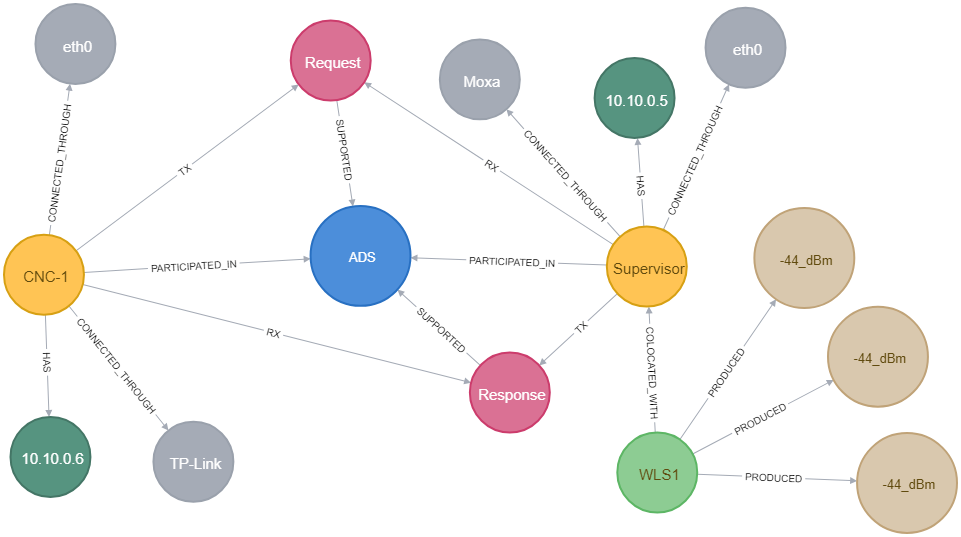
\includegraphics[width=0.95\textwidth]{./chapter-gdb-appl/figures/database/graph_Single_trans.png}
    \caption{A detailed visualization resulting from a testbed experiment for all the nodes and relationships corresponding to a single transaction. }
    \label{gdbappl:fig::Sample-graph_2}
\end{figure}

\subsection{Calculation of Metrics}

\begin{figure}[!ht]
	\centering
%	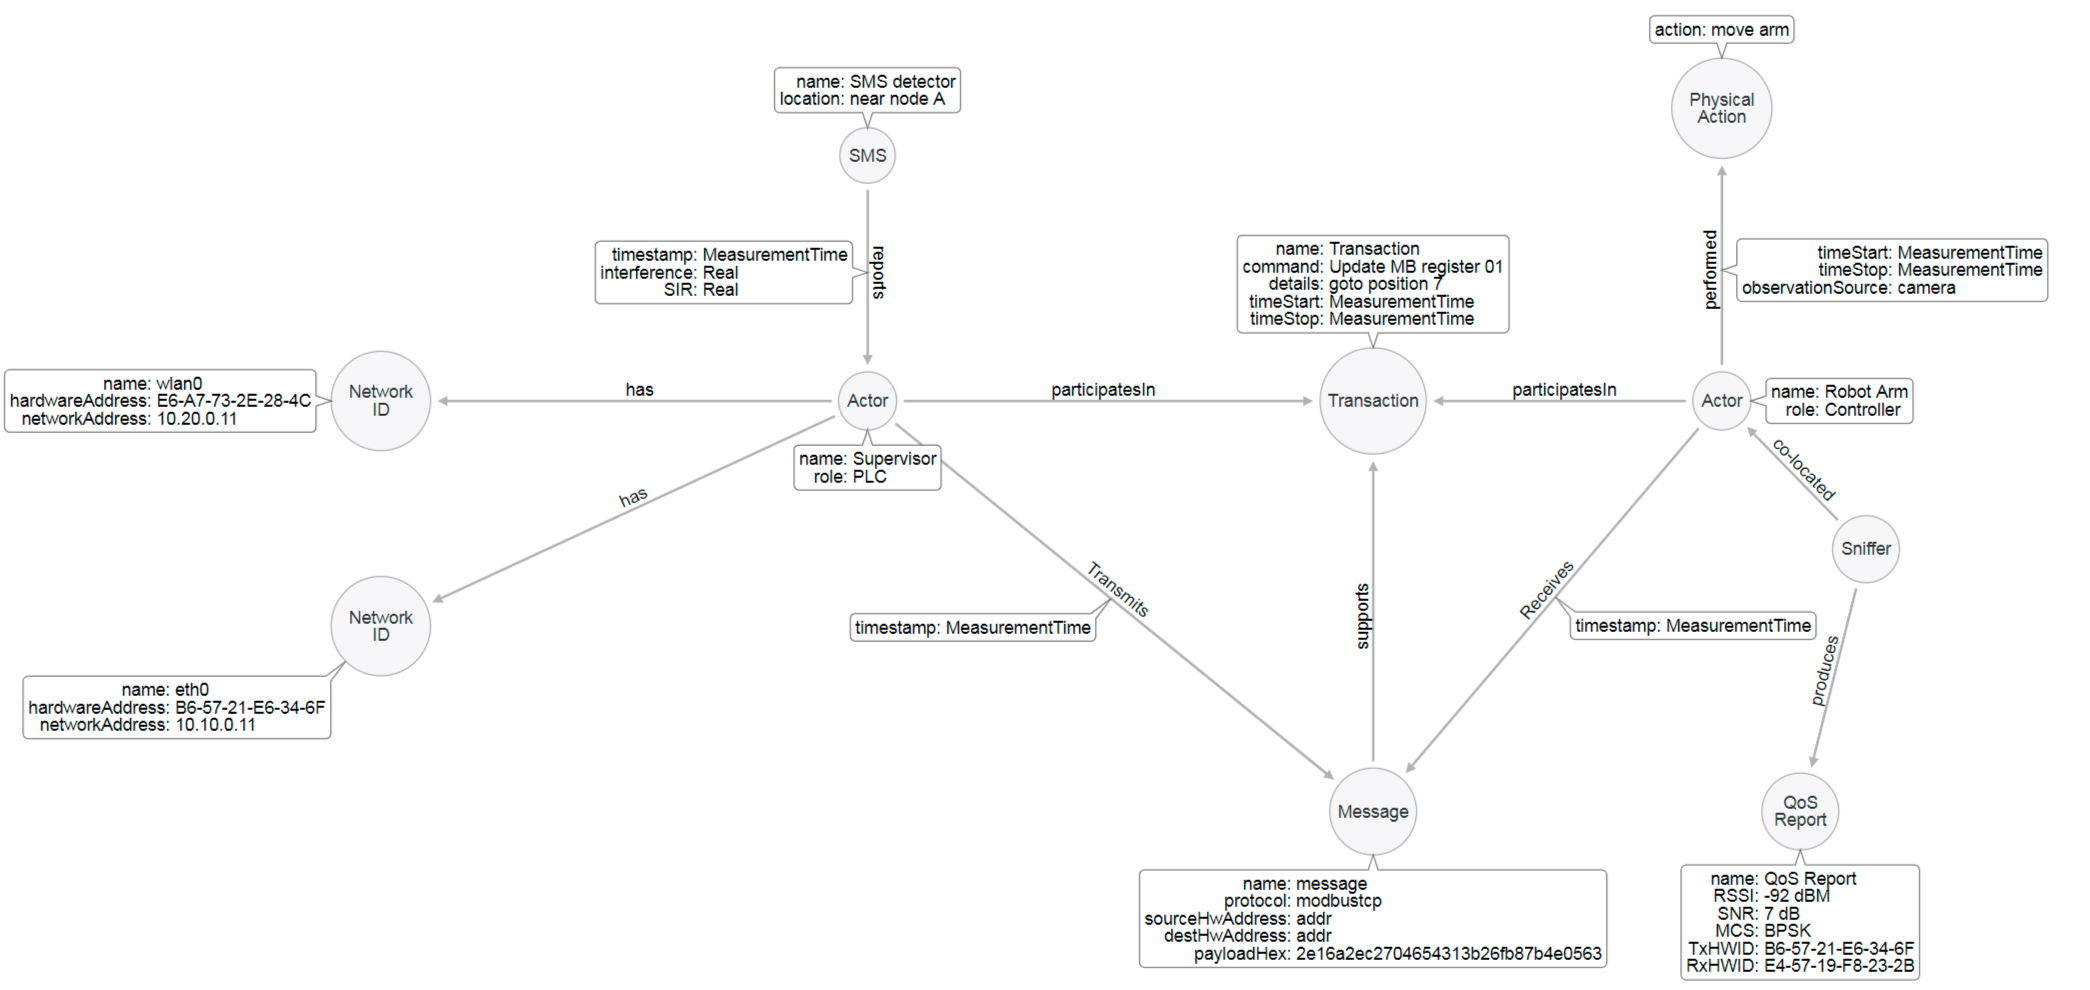
\includegraphics[width=\textwidth,trim=50 50 50 50, clip]{figures/database/arrows-schema.PNG}
	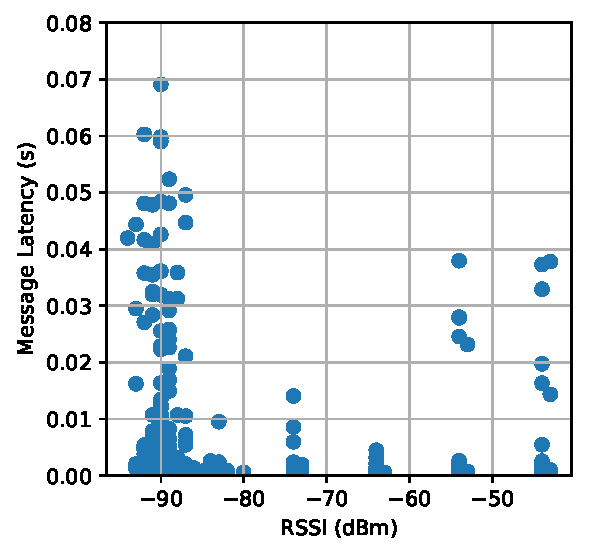
\includegraphics[width=0.5\textwidth]{./chapter-gdb-appl/figures/database/scatter_1.eps}
	\caption{Correlation between the message latency and the RSSI values by the sniffer.}
	\label{gdbappl:fig::database:scatter}
\end{figure}

We now present an example of deploying the proposed GDB approach in industrial wireless analysis. During the trial run time, we varied an RF attenuator value in the single wireless link. The attenuation can take the values \{0, 10, 20, 30, 40, 50, 60\} dB. We evaluate the message latency as the difference between the receive and transmit times of a message including transmission, processing, and retransmission times. Each message has been coupled to a QoS report that is the one reported at the closest time instant before the message transmit time. One of the parameters in the QoS report is the RSSI value captured by the Sniffer colocated with the supervisor's wireless adapter. 

In Fig.~\ref{gdbappl:fig::database:scatter}, we present a scatter plot showing the correlation between the message latency in seconds to the measured RSSI values by the sniffer in dBm.  The figure shows that the latency is higher at the lower RSSI values due to the increased number of retransmissions. Generally, an IEEE 802.11 transmission can occur using different IEEE 802.11 mode and modulation and coding scheme (MCS) based on the channel quality. At the RSSI of -90 dBm, the receiver should operate at the most robust communications mode and the lowest MCS index. However, retransmissions still occur due to having the received power near the sensitivity of the supervisor's wireless adapter. As shown in Fig.~\ref{gdbappl:fig::database:scatter}, retransmissions may occur at other RSSI values as well when the transmitter selects a higher mode of transmission and a higher MCS index. In this case, we assert that the receiver is operating close to the marginal sensitivity for a given mode (e.g., 802.11n) and MCS index.  We observed that the transmitter switches to a lower MCS index for the retransmitted messages, which supports our supposition. Therefore, latency can in fact be high for better RSSI values.  This effect is illustrated in Fig.~\ref{gdbappl:fig::database:scatter} where certain messages can have latency values at -43 dBm, which are comparable to those in the case of  -90 dBm.  

%SAMPLE CALCULATION FOR REDUCED GRAPH SHOWN ABOVE OVER A SMALL PERIOD OF TIME
%* network delay
%* correlate power level to delay
%* show the cypher command for computing this stuff

%TALK ABOUT LATER: SAMPLE CALCULATION OF PERFORMANCE DEPENDENCY OF THROUGHPUT TO NETWORK PERFORMANCE ON A SLIDING WINDOW

\section{Future Direction}

We have presented the general architecture of a performance evaluation database.  Future work will include developing query algorithms for the calculation of performance metrics as well as correlation of network events to the physical performance of the manufacturing system.  Algorithms will be developed to indicate locations in time of lost information making more direct performance correlations possible.  Beyond performance evaluation of the manufacturing system, we believe that the graph database approach enables anomaly detection because relationships within the data are intrinsically stored and thus efficiently queried.  The structure of the information is important within a graph database, and defining the relationships such that the paths through nodes may be discovered is essential to efficient queries and discovery of hidden correlations.  Therefore, more research will be done in the modification of the presented schema.  Machine learning will be applied for the detection of anomalies, performance degradation, signal quality, and network performance enhancement through more efficient resource allocation.  Our plans also include online database insertions to enable the demonstration of online operation of the database.   We also intend to examine the development of better control system strategies that mitigate network losses and delays.  Since this approach is indifferent to the communications  protocols used, we intend to extend our database approach to include various protocols, radio bands such as millimeter wave bands for 5G communications, and different use cases to include mobile robotic platforms and safety critical systems.

\section{Conclusions} \label{gdbappl:sec::conclusion}
We have presented in this paper a novel approach to capturing network and operational event information from a factory workcell with the  purposes of 1) capturing and storing of network and operational events, 2) calculating performance metrics of the network, and 3) discovering performance dependencies between the network and the physical assembly of the workcell.  Using a graph database, we have demonstrated that it is possible to construct such a database, compute network performance metrics and discover correlations.  We have also developed the capability of examining the correlation between network events and the performance of physical actions.  This will be a source of further research.

Future progress and measurement data will be deposited in the NIST public domain repository as a reference for industrial traffic modeling efforts and comparative studies on industrial wireless technologies~\cite{Candell2019PROJECTURL}.



% references section
%\bibliography{chapter-gdb-appl/gdb-appl}
